\subsection{Fusion nucléaire}
 
\begin{frame}{Fusion nucl\'eaire Magn\'etique: ITER}
\small
\begin{columns}
\begin{column}{5.5cm}
\begin{itemize}
\only<1>{
\item \textbf{Fission nucl\'eraire}: production d'\'energie en utilisant la fission d'atomes lourds (uranium) par bombardement de neutrons (nucl\'eaire civil actuel).
\vspace{1mm}
\item \textbf{Fusion DT}: \`a de tr\`es hautes \'energies  le deuterium et tritium (hydrog\`ene) fusionnent en d\'egageant de l'\'energie (r\'eaction pr\'esente dans les \'etoiles).
\vspace{1mm}
\item \textbf{Plasma}: \`a de tr\`es hautes temp\'eratures  la ionisation du gaz donne un plasma (gaz charg\'e) sensible au champ magn\'etique et \'electrique.
}
\only<2>{
\item \textbf{Tokamak}: Chambre toro\"{i}dale utilis\'ee pour confiner le plasma avec un champ magn\'etique.
\item \textbf{ITER}: Projet international de r\'eacteur exp\'erimental ayant pour but de valider la fusion comme source d'\'energie.
\item \textbf{Petit histoire d'ITER}: Projet propos\'e par R. Reagan et M. Gorbatchev en 1985. Le trait\'e final fut sign\'e en 2006.
\item \textbf{ITER en chiffre}: 34 pays (UE, USA, Chine, Russie, Inde, Cor\'ee, Japon). Construction: 12 ans et 13 Milliards de co\^{u}t.  Exploitation: 20 ans et 5 Mds. 
}
\end{itemize}
\end{column}
\begin{column}{8.5cm}
\only<1>{
\begin{figure}
 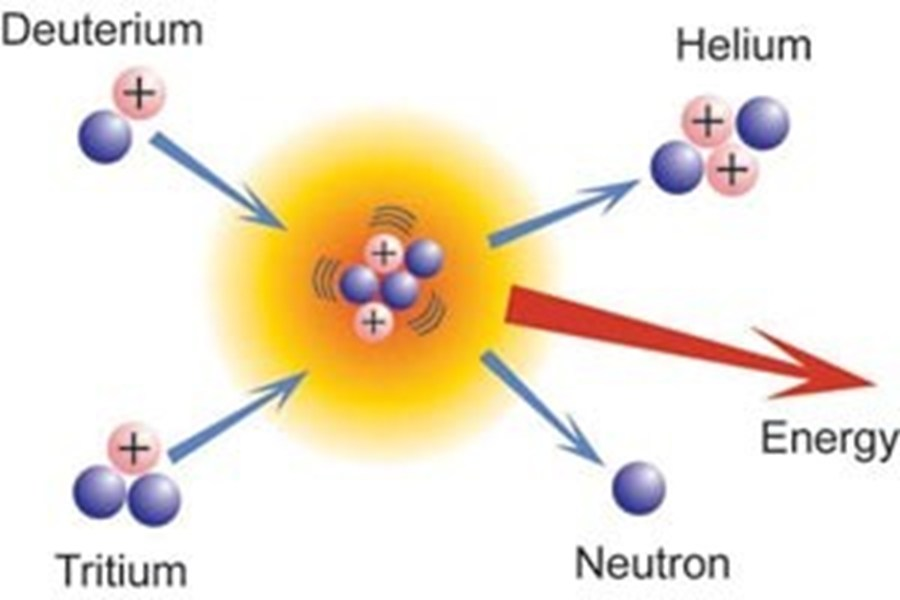
\includegraphics[width=.7\linewidth]{fusion_reaction.jpg}
\end{figure}
}
\only<2>{
\begin{figure}
 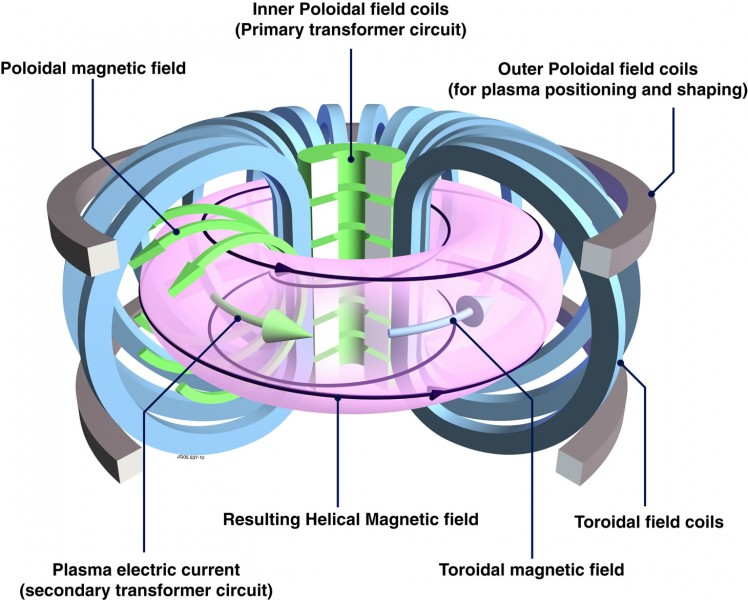
\includegraphics[width=.8\linewidth]{Tokamak.jpg}
\caption{\scriptsize Tokamak}
\end{figure}
}
\end{column}
\end{columns}
\end{frame}


\begin{frame}{Fusion Vs Fission nucl\'eaire}
\small
\begin{columns}
\begin{column}{6cm}
\textbf{Fission Nucl\'eaire}:
\begin{itemize}
\item Avantages
\begin{itemize}
\item Co\^{u}t comp\'etitif, 
\item Pas d'\'emission de CO 2.
\end{itemize}
\item Inconv\'enients
\begin{itemize}
\item Combustible (uranium) limit\'e.
\item D\'echets radioactif \`a grande longue dur\'ee de vie (traitement compliqu\'e et co\^{u}teux.
\item Risque d'accident critique (r\'eaction en chaine etc) type Tchernobyl ou Fukushima.
\end{itemize}
\end{itemize}
\end{column}
\begin{column}{6cm}
\textbf{Fusion Nucl\'eaire}
\begin{itemize}
\item Avantages
\begin{itemize}
\item Enorme r\'eserve de combustible.
\item Pas d'\'emission de CO 2.
\item Peu de d\'echets et \`a faible dur\'ee de vie.
\item Pas de risque d'accident critique.
\end{itemize}
\item Inconv\'enients
\begin{itemize}
\item On sait pas maitriser cette source d'\'energie. Confiner un plasma a 100 millions de degr\'es g\'en\`ere des difficult\'es \'enormes.  
\end{itemize}
\end{itemize}
\end{column}
\end{columns}
\end{frame}


\begin{frame}{Mod\'elisation du plasma I}
  \small
  \begin{itemize}
\item Premier mod\`ele: \textbf{\'equation de Vlasov-Maxwell} qui d\'ecrit l'\'evolution de la fonction de distribution des particules (description statistique du plasma).
\begin{block}{Vlasov-Maxwell}
On d\'efinit $f(t,\mathbf{x},\mathbf{v})$ la distribution  des particules charg\'ees. 
$$
\left\{\begin{array}{l}
\partial_t f +\mathbf{v}\cdot\nabla_{\mathbf{x}} f+ \frac{q}{m}\left(\mathbf{E}+\mathbf{v}\times\mathbf{B}\right)\cdot\nabla_{\mathbf{v}} f= Q(f,f)\\
 \frac{1}{c^2}\partial_t \mathbf{E}-\nabla \times \mathbf{B}= -\mu_0\mathbf{J},\\
\partial_t \mathbf{B}=-\nabla \times \mathbf{E},\quad \nabla \cdot\mathbf{B}=0,\quad \nabla \cdot \mathbf{E} =\frac{\sigma}{\varepsilon_0}.
\end{array}\right.
$$
avec $Q$ l'op\'erateur de collision, $\mathbf{E}$, $\mathbf{B}$ les champs \'electrique et magn\'etique et $\mathbf{J}$ le courant.
\end{block}
\item Mod\`ele  pour les plasmas peu collisionnels (coeur du tokamak).
\item \textbf{Probl\`emes num\'eriques} :  \'equation 6D et physique multi-\'echelle ce qui g\'en\`ere  d'\'enorme co\^{u}t de calcul.
\item \textbf{Recherches}: m\'ethodes num\'eriques pr\'ecises et moins co\^{u}teuses.
\end{itemize}
\end{frame}

\begin{frame}{Mod\'elisation du plasma II}
  \small
  \begin{itemize}
\item Second mod\`ele: \textbf{\'equation de la MHD} qui d\'ecrit l'\'evolution du plasma \a l'aide des quantit\'es macroscopiques.
\begin{block}{MHD}
$$
  \left\{\begin{array}{l}
\partial_t \rho+\nabla\cdot(\rho\mathbf{u})=0,\\
\rho\partial_t \mathbf{u}+\rho\mathbf{u}\cdot\nabla \mathbf{u}+\nabla p=\mathbf{J}\times\mathbf{B}+\textcolor{blue}{\nu \triangle \mathbf{u}}\\
\partial_t p+\mathbf{u}\cdot\nabla p+\gamma p\nabla\cdot \mathbf{u}=\textcolor{blue}{\nabla \cdot (K \nabla T)}\\
\partial_t \mathbf{B}=\nabla \times \left(\mathbf{u}\times\mathbf{B}-\textcolor{blue}{\eta\mathbf{J}}\right),\\
\nabla\cdot\mathbf{B}=0, \quad \nabla\times\mathbf{B}= \mathbf{J}.
\end{array}\right.
$$
avec $\rho$, $\mathbf{u}$, $T$ et $p$ la densit\'e, la vitesse, la temp\'erature et la pression du plasma.
\end{block}
\item Mod\`ele  pour les plasmas tr\`es collisionnels (bords du tokamak).
\item \textbf{Probl\`emes num\'eriques} :  Mod\`ele complexe et physique multi-\'echelle 
\item \textbf{Recherches}: m\'ethodes num\'eriques  peu co\^{u}teuses pr\'eservant les propri\'et\'es du mod\`ele (exemple: positivit\'e).
\end{itemize}
\end{frame}

\begin{frame}{Applications : instabilit\'es de bord}
\small
\begin{columns}
\begin{column}{6.5cm}
\begin{itemize}
\item Les gradients  de pression au bords peuvent occasionner des ruptures de confinement sous forme d'instabilit\'es.
\item Exemples: 
\begin{itemize}
\item \textbf{Disruptions}: Instabilit\'es du plasma brutale pouvant endommager de fa\c{c}on critique le Tokamak.
\item \textbf{Edge localized modes (ELMs)}: Instabilit\'es de bord p\'eriodiques  pouvant endommager le tokamak et g\'en\'erant un perte d'\'energie.
\end{itemize}
\vspace{1mm}
\item \textcolor{red}{La simulation num\'erique permet de comprendre ces instabilit\'es, les estimer et tester des m\'ethodes de contr\^{o}le}. 
\end{itemize}
\end{column}
\begin{column}{7.5cm}
\begin{itemize}
\item Simulation d' ELm's 
\end{itemize}
\only<1>{
\begin{figure}
 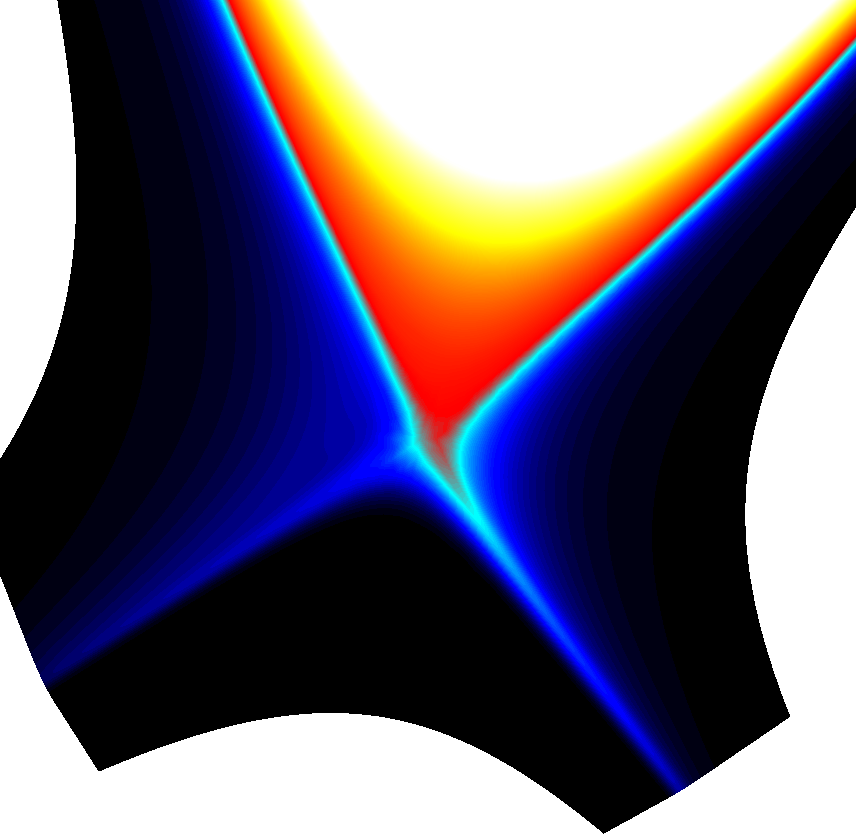
\includegraphics[width=.65\linewidth]{elm-movie/elm-pressure-movie_1400x1070_0000.png}
\end{figure}
}
\only<2>{
\begin{figure}
 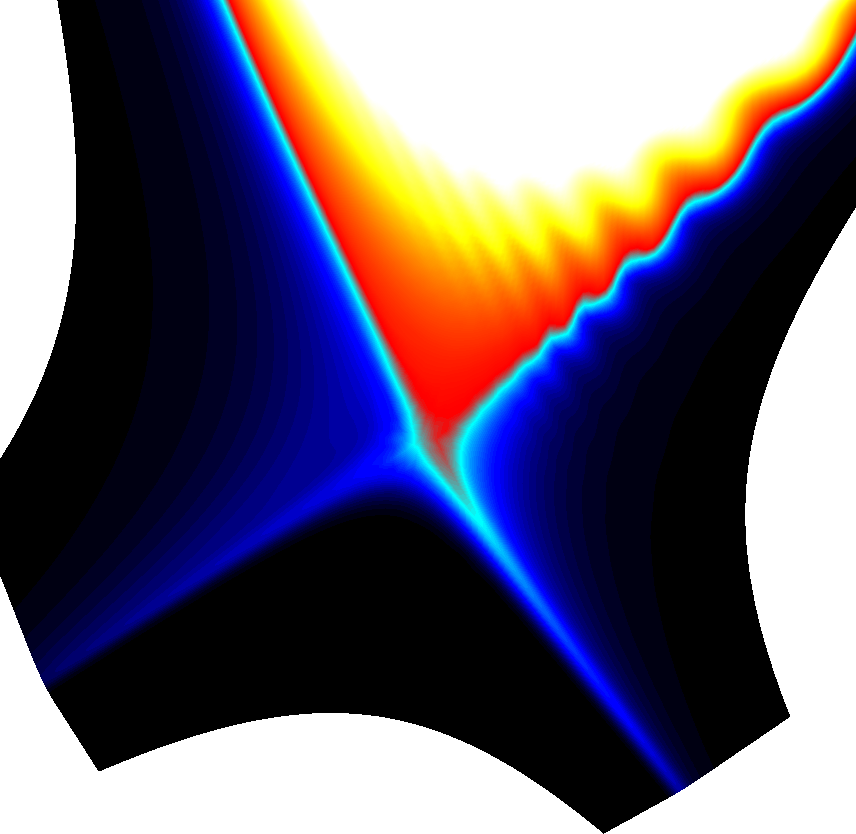
\includegraphics[width=.65\linewidth]{elm-movie/elm-pressure-movie_1400x1070_0050.png}
\end{figure}
}
\only<3>{
\begin{figure}
 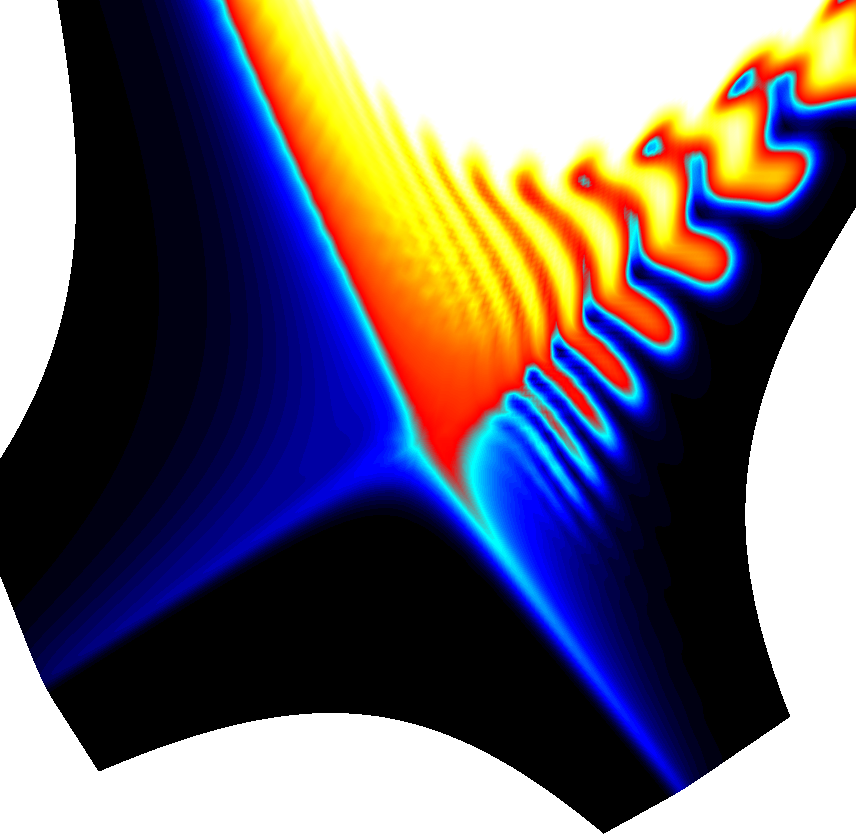
\includegraphics[width=.65\linewidth]{elm-movie/elm-pressure-movie_1400x1070_0100.png}
\end{figure}
}
\only<4>{
\begin{figure}
 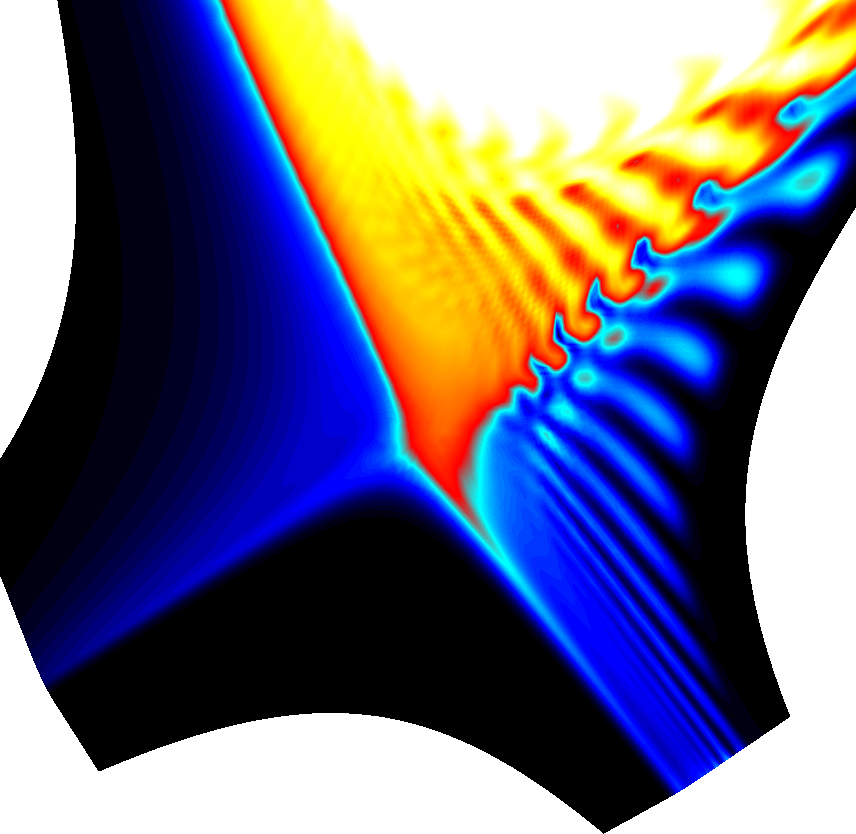
\includegraphics[width=.65\linewidth]{elm-movie/elm-pressure-movie_1400x1070_0150.png}
\end{figure}
}
\only<5>{
\begin{figure}
 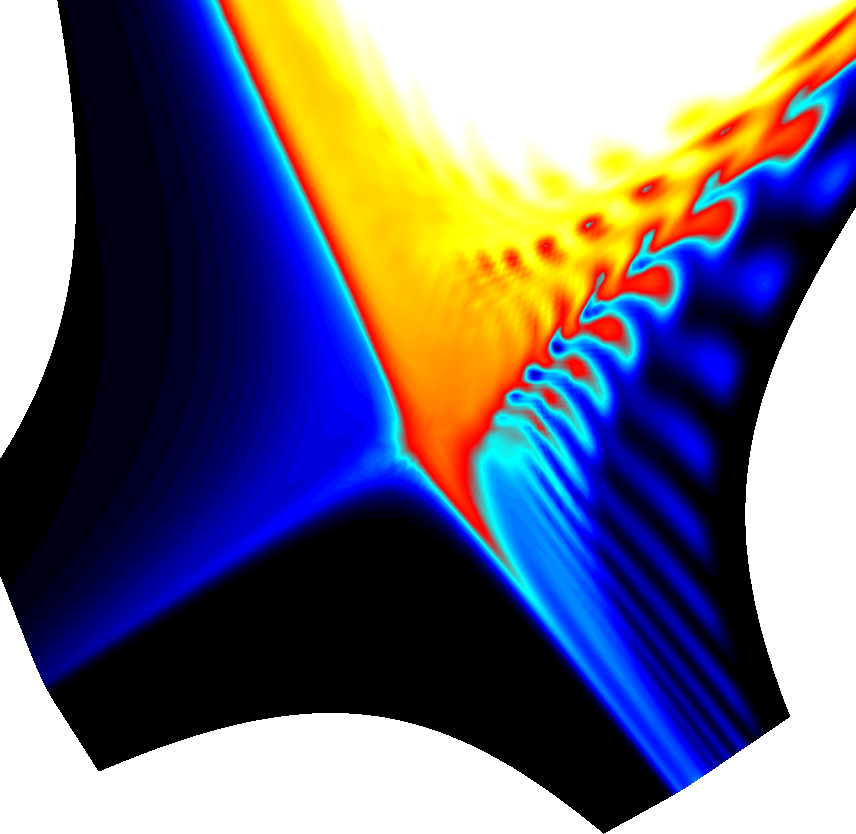
\includegraphics[width=.65\linewidth]{elm-movie/elm-pressure-movie_1400x1070_0200.png}
\end{figure}
}
\only<6>{
\begin{figure}
 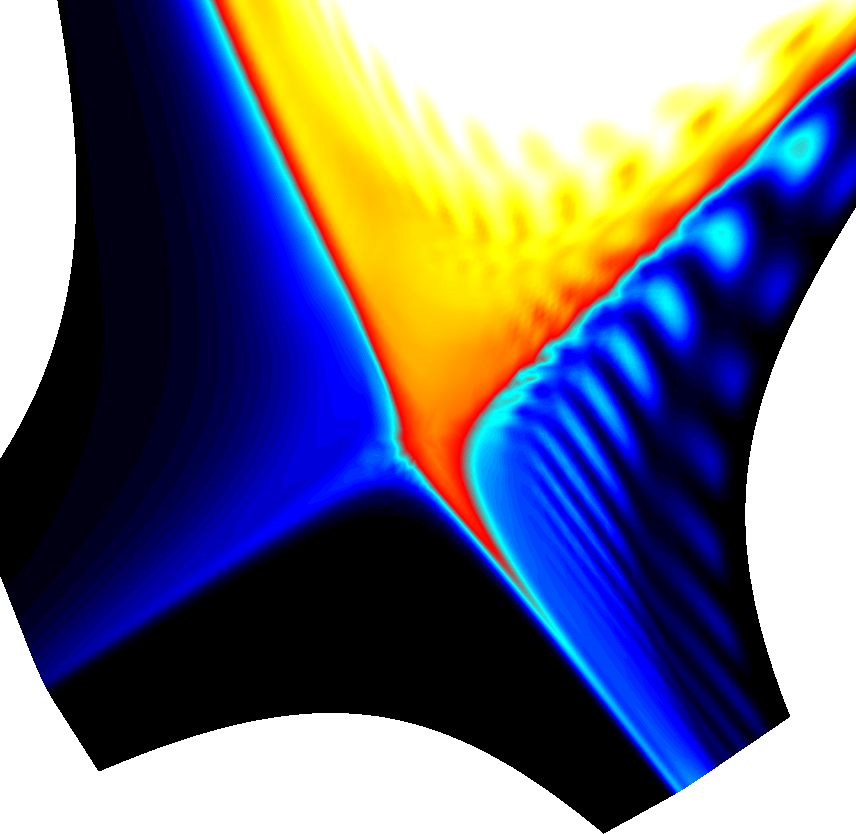
\includegraphics[width=.65\linewidth]{elm-movie/elm-pressure-movie_1400x1070_0250.png}
\end{figure}
}
\end{column}
\end{columns}
\end{frame} 

%%% Local Variables: 
%%% mode: latex
%%% TeX-master: "slides-math-formations-metiers"
%%% End: 
